% !TEX program = XeLaTeX
% !TEX encoding = UTF-8
\documentclass[UTF8,nofonts]{article}
%{ctexart}




\usepackage[T1]{fontenc}
\usepackage[utf8x]{inputenc}
\usepackage[english,portuguese]{babel}




%\setCJKmainfont[BoldFont=FandolSong-Bold.otf,ItalicFont=FandolKai-Regular.otf]{FandolSong-Regular.otf}
%\setCJKsansfont[BoldFont=FandolHei-Bold.otf]{FandolHei-Regular.otf}
%\setCJKmonofont{FandolFang-Regular.otf}




\usepackage{lipsum}
\usepackage{url}
\usepackage{cancel}
\usepackage{xspace}
\usepackage{graphicx}
\usepackage{multicol}
\usepackage{multirow}
\usepackage{subfig}
\usepackage{amsmath}
\usepackage{amssymb}
\usepackage[a4paper, width=186mm, top=18mm, bottom=18mm, includeheadfoot]{geometry}
%\usepackage[a4paper, width=140mm, top=18mm, bottom=22mm, includeheadfoot]{geometry}
\usepackage{booktabs}
\usepackage{array}
\usepackage{verbatim}
\usepackage{caption}
\usepackage{natbib}
\usepackage{booktabs}
\usepackage{float}
\usepackage{pdflscape}
\usepackage{mathtools}
\usepackage[usenames, dvipsnames]{xcolor}
\usepackage{afterpage}
\usepackage{pgf}
\usepackage{tikz}
\usepackage{dirtree}
\usepackage[style=american]{csquotes}
\usepackage{amsfonts}
\usepackage{tikz}
\usepackage{tkz-graph}
\usetikzlibrary{arrows,decorations.pathmorphing,automata,positioning,backgrounds,fit,shapes.symbols,chains,intersections}

\newtheorem{definition}{Definition}[section]
\newtheorem{theorem}{Theorem}[section]
\newtheorem{lemma}{Lemma}
\newtheorem{proof}{Proof} [section]



\usepackage[toc, page, title, titletoc, header]{appendix}
\usepackage{marginnote}
\usepackage{tablefootnote}

%\renewcommand\appendixname{附\ 录}
%\renewcommand\appendixpagename{附\ 录}
%\renewcommand\appendixtocname{附\ 录}
\renewcommand\abstractname{Abstract}


\usepackage{perpage} %the perpage package
\MakePerPage{footnote} %the perpage package command

\usetikzlibrary{shapes.geometric}%
\usepackage{color}
%\usepackage[pages=some, placement=top]{background}
\usepackage{eso-pic}
\usepackage[final]{pdfpages}

%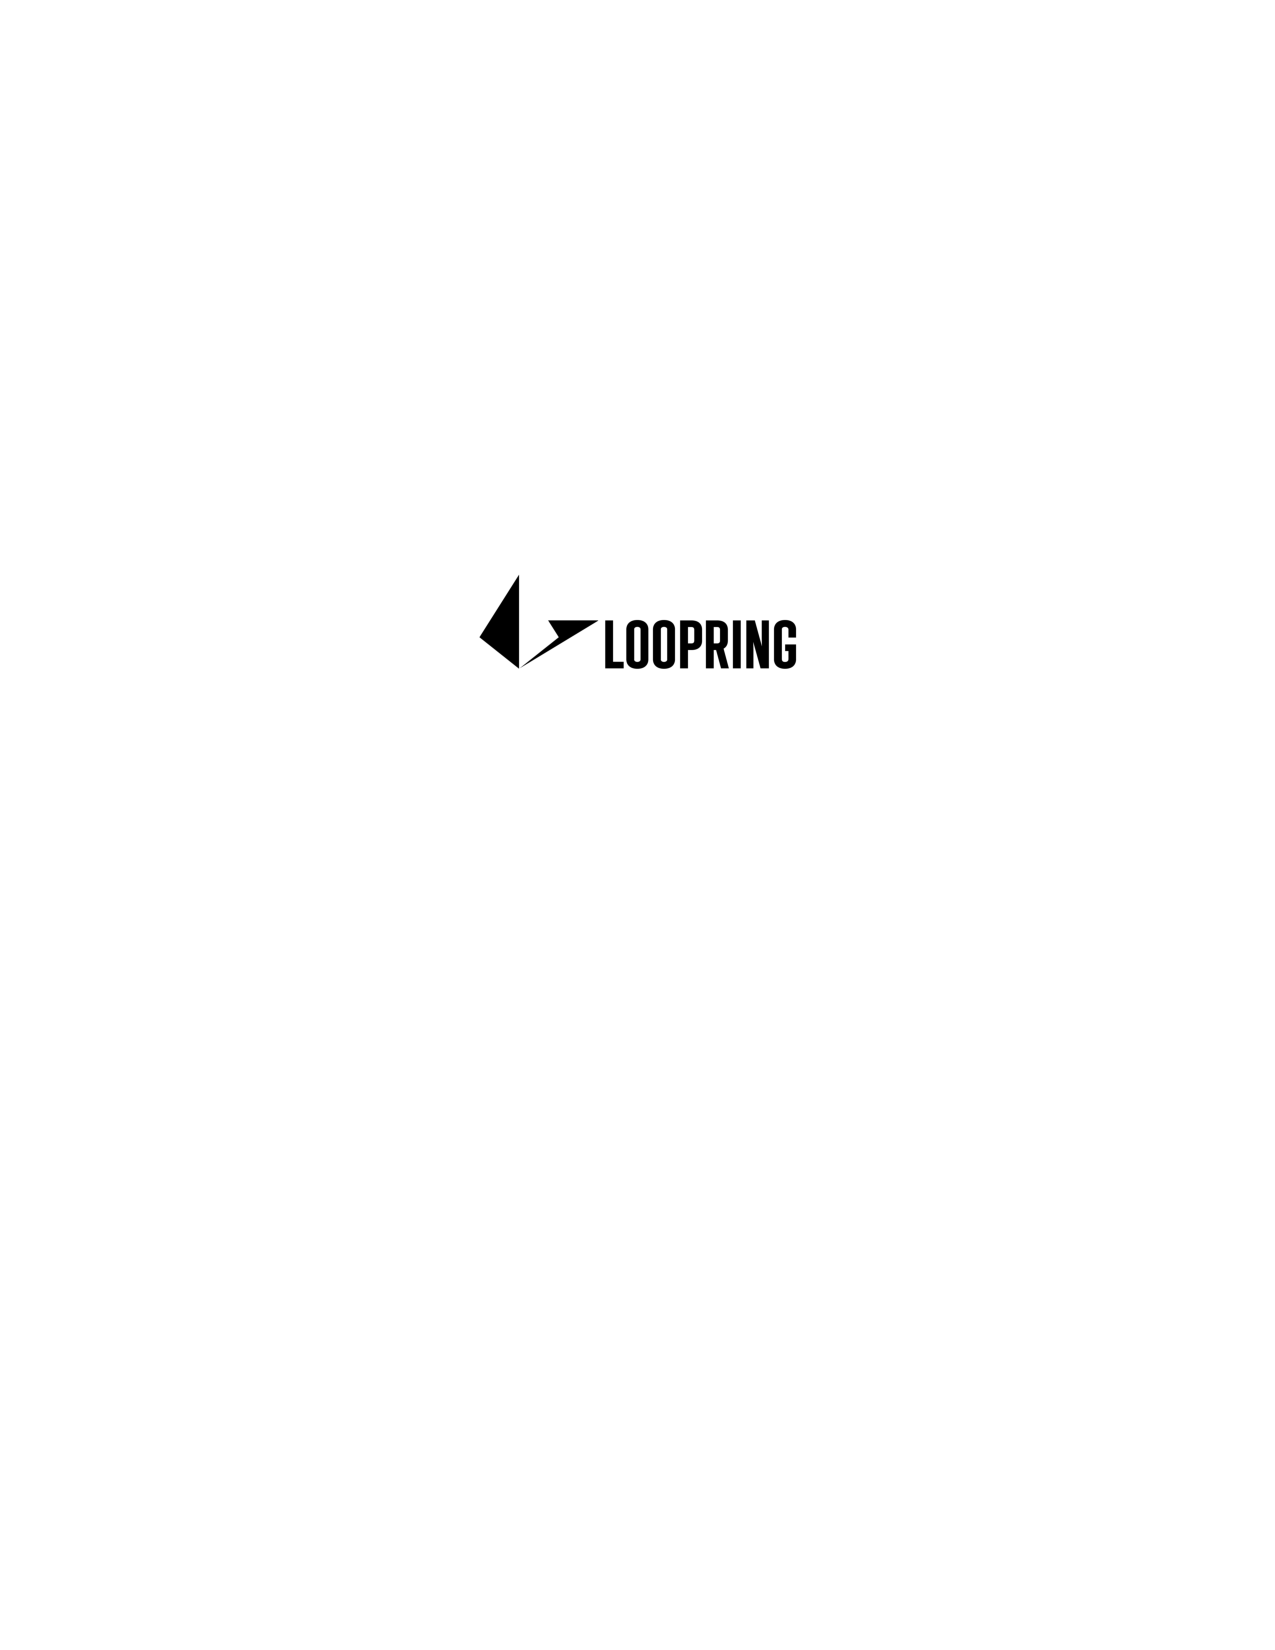
\includepdf[pages=1]{cover}
\hyphenpenalty=750

\title{\textbf{Loopring:}\\\textbf{Protocolo para Exchanges Descentralizadas}}
\author{
  Daniel Wang\\
  \texttt{daniel@loopring.org}\\
  \and
  	Jay Zhou\\
  	\texttt{jay@loopring.org}\\
  	\and
  	Alex Wang\\
  	\texttt{alex@loopring.org}\\
  	\and
  	Matthew Finestone\\
  	\texttt{matt.finestone@gmail.com}\\ 
  \\
  \texttt{https://loopring.org}
 }

\makeatletter
\def\CTEX@section@format{\Large\bfseries}
\makeatother

\makeatletter
\newenvironment{tablehere}
 {\def\@captype{table}}
 {}

\newenvironment{figurehere}
 {\def\@captype{figure}}
 {}
\makeatother
%
%\newcommand\BackgroundPic{%
%\put(0, 0){%
%\parbox[b][\paperheight]{\paperwidth}{%
%\vfill
%\centering
%\includegraphics[width=\paperwidth, height=\paperheight, %
%%keepaspectratio]{images/background.jpg}%
%]{images/background.jpg}%
%\vfill
%}}}


\begin{document}
%\AddToShipoutPicture{\BackgroundPic}
\maketitle


\begin{abstract}
Loopring é um protocolo aberto para a construção de exchanges descentralizadas. Loopring opera como um conjunto público de contratos inteligentes responsáveis pela negociação (trader) e liquidação, com um grupo de agentes off-chain agregando e comunicando pedidos. O protocolo é gratuito, extensível e serve como um bloco de construção padronizado para aplicativos descentralizados (dApps) que incorporam a funcionalidade de exchange. Seus padrões interoperáveis facilitam a negociação anônimo e sem confiança. Uma melhoria importante em relação aos atuais protocolos de exchanges descentralizadas é a capacidade de os pedidos serem misturados e combinados com outros pedidos diferentes, eliminando as restrições dos pares de negociação de dois tokens e melhorando drasticamente a liquidez. A Loopring também emprega uma solução única e robusta para impedir o front-running: a tentativa injusta de enviar transações para um bloco mais rápido do que o provedor da solução original. Loopring é independente de blockchain e implementável em qualquer blockchain com funcionalidade de contrato inteligente. Nesse momento, é operável na Ethereum\cite{buterin2017ethereum} \cite{wood2014ethereum} e Qtum \cite{dai2017smart} com NEO \cite{atterlonn2018distributed} em construção.
\end{abstract}



\begin{multicols}{2}
\section{Introdução\label{sec:introduction}}

Com a proliferação de ativos baseados em blockchain, a necessidade de trocar esses ativos entre as contrapartes aumentou significativamente. À medida que milhares de novos tokens são introduzidos - incluindo a tokenização de ativos tradicionais - essa necessidade é ampliada. Seja motivado por negociações de tokens especulativos, ou convertendo para acessar redes através de seus tokens de utilidade nativos, a capacidade de trocar um cripto por outro é fundamental para o ecossistema maior. De fato, existe uma energia potencial em ativos \cite{desotocapital}, e a realização desse capital de desbloqueio de energia - requer não apenas a afirmação de propriedade, que as blockchains impediram imensamente, mas a capacidade de transferir e transformar livremente esses ativos.
 
Assim sendo, a negociação sem confiança de tokens (valor) é um caso de uso atraente para a tecnologia blockchain. 
Até agora, no entanto, os entusiastas cripto decidiram amplamente fazer negociação de seus tokens em exchanges centralizadas tradicionais. O protocolo Loopring é necessário porque, assim como o Bitcoin \cite{nakamoto2008bitcoin} respeitosamente enfatizou que, em relação ao dinheiro eletrônico peer-to-peer, \enquote{os principais benefícios são perdidos se um terceiro confiável ainda for necessário para evitar gastos duplicados}, Da mesma forma, os principais benefícios dos ativos descentralizados são perdidos se eles precisarem passar por exchanges confiáveis, fechadas e centralizadas. 
Fazer negociação de tokens descentralizados em exchanges centralizadas não faz sentido do ponto de vista filosófico, já que falha em defender as virtudes que esses projetos descentralizados adotam. Há também inúmeros riscos e limitações práticas no uso de exchanges centralizadas, descritas abaixo. Exchanges Descentralizadas (Decentralized Exchanges - DEXs) \cite{schuh2015bitshares} \cite{bancor} \cite{kyber} procuraram abordar essas questões e, em muitos casos, conseguiram aliviar os riscos de segurança usando blockchains para desintermediação. No entanto, como a capacidade do DEX torna-se uma infraestrutura crucial para a nova economia, há espaço substancial para a melhoria do desempenho. O Loopring visa fornecer ferramentas modulares para essa infraestrutura com seu protocolo aberto agnóstico do dApp.

\section{Cenário atual das Exchange\label{sec:current_exchange_landscape}}

\subsection{Inadequações das Exchanges Centralizadas}
Os três principais riscos das exchanges centralizadas são; 1) Falta de segurança, 2) Falta de transparência e 3) Falta de liquidez.

\textbf{Falta de Segurança} surge de usuários que entregam o controle de suas chaves privadas (fundos) a uma entidade centralizada. Isso expõe os usuários à possibilidade de que as exchanges centralizadas sejam vítimas de hackers mal-intencionados. Os riscos de segurança e hackers que enfrentam todas as exchanges centralizadas são bem conhecidos \cite{coincheckhack}  \cite{mcmillan2014inside}, ainda são muitas vezes aceitos como \enquote{table stakes (mesa de apostas)} para o negociador de tokens. As exchanges centralizadas continuam a ser chamariz para os hackers atacarem, pois seus servidores custodiam milhões de dólares em fundos de usuários. Os desenvolvedores das exchanges também podem cometer erros acidentais e sem más intenções com os fundos do usuário. Simplesmente, os usuários não estão no controle de seus próprios tokens quando depositados em uma exchange centralizada.

\textbf{Falta de Transparência} expõe os usuários ao risco de exchanges desonestas que agem de forma injusta. A distinção aqui é pelas intenções maliciosas da exchange, já que os usuários não estão realmente negociando seus próprios ativos em exchanges centralizadas, mas sim, uma nota promissória. Quando os tokens são enviados para a carteira da exchange, a exchange fica sob custódia e oferece uma nota promissória em seu lugar. Todos os negócios são efetivamente entre as notas promissórias dos usuários. Para retirar seus fundos, os usuários resgatam suas notas promissórias com a exchange e recebem seus tokens em seu endereço de carteira externa. Ao longo deste processo, há uma falta de transparência, e a exchange pode paralisar, congelar sua conta, ir à falência, etc. Também é possível que eles usem ativos dos usuários para outros fins enquanto estão sob custódia, como cedê-los a terceiros. A falta de transparência pode custar muito aos usuários mesmo sem uma perda total de fundos, como taxas de negociação mais altas, atrasos quando houver alta demanda, risco regulatório e pedidos em execução.

\textbf{Falta de Liquidez.} Do ponto de vista dos operadores da exchange, a liquidez fragmentada inibe a entrada de novas exchanges por causa de dois cenários, "o vencedor leva tudo". Primeiro, a exchange com o maior número de pares de negociação ganha, porque os usuários acham mais fácil fazer todas suas negociações em uma única exchange. Em segundo lugar, a exchange com o maior livro de ofertas (order book) vence, devido a spreads favoráveis de compra-venda para cada par de negociação. Isso desencoraja a concorrência dos recém-chegados, porque é difícil para eles acumular liquidez inicial. Como resultado, muitas exchanges geram uma alta participação de mercado, apesar das queixas dos usuários e até mesmo grandes incidentes de hackers. Vale a pena notar que, à medida que as exchanges centralizadas ganham market share, elas se tornam um alvo cada vez maior de hackers.

Do ponto de vista dos usuários, a liquidez fragmentada reduz significativamente a experiência do usuário. Em uma exchange centralizada, os usuários só podem negociar dentro das próprias pools de liquidez da exchange, contra seu próprio livro de ofertas e entre seus pares de token suportados. Para negociar o token \verb|A| para o token \verb|B|, os usuários devem ir a uma exchange que suporte os dois tokens ou registrar-se em diferentes exchanges, divulgando informações pessoais. Os usuários geralmente precisam executar negociações preliminares ou intermediárias, normalmente contra o BTC ou ETH, pagando spreads no processo de compra e venda. Finalmente, os livros de ofertas podem não ter liquidez o suficiente para concluir o negócio. Mesmo que a exchange pretenda processar grandes volumes, não há garantia de que esse volume e liquidez não sejam falsos \cite{fakevolume}.

O resultado são silos de liquidez desconexos e um ecossistema fragmentado que se assemelha ao legado sistema financeiro, com volume de negociação significativamente centralizado em poucas exchanges. As promessas de liquidez global das blockchains não têm mérito dentro de exchanges centralizadas.

\subsection{Inadequações das Exchanges Descentralizadas}
As exchanges descentralizadas diferem das exchanges centralizadas em parte porque os usuários mantêm o controle de suas chaves privadas (ativos) executando negociações diretamente no blockchain subjacente. Ao alavancar a tecnologia sem confiança das criptomoedas, elas mitigam com sucesso muitos dos riscos acima mencionados relacionados à segurança. No entanto, persistem problemas em relação ao desempenho e limitações estruturais. 

A liquidez muitas vezes continua sendo um problema, pois os usuários devem buscar contrapartes em diferentes pools e padrões de liquidez. Os efeitos de liquidez fragmentada estão presentes se os DEXs ou os dApps em geral não empregarem padrões consistentes para interoperar e se os pedidos não forem compartilhados/propagados em uma rede ampla. A liquidez dos livros de ofertas e, especificamente, sua resiliência - a rapidez com que as ordens de limite são regeneradas - podem afetar significativamente as estratégias de negociação ideais \cite{limitorderliquidity}. A ausência de tais padrões resultou não apenas em liquidez reduzida, mas também exposição a uma série de contratos inteligentes proprietários potencialmente inseguros.

Além disso, como as negociações são realizados na blockchain, as DEXs herdam as limitações da blockchain subjacente, a saber: escalabilidade, atrasos na execução (mineração) e modificações dispendiosas nas ordens. Assim, os livros de ofertas blockchain não são particularmente adequados, já que a execução de código na blockchain incorre em um custo (gás), tornando a opção de cancelamento de pedidos muito caras. 

Finalmente, como os livros de ofertas blockchain são públicos, a transação para fazer um pedido é visível para os mineiradores enquanto aguarda a mineração para o próximo bloco e colocados em um livro de ofertas. Esse atraso expõe o usuário ao risco de ter o preço ou a execução se movendo contra ele.

\subsection{Soluções Híbridas}
Pelas razões acima, as exchanges puramente baseadas em blockchain têm limitações que as tornam pouco competitivas em exchanges centralizadas. Existe uma compensação entre a confiabilidade inerente on-chain e a velocidade de uma exchange centralizada e a flexibilidade do pedido. Protocolos, como Loopring e 0x \cite{warren20170x} estendem uma solução de liquidação on-chain com o gerenciamento de pedidos off-chain. Essas soluções giram em torno de contratos inteligentes abertos, mas navegam pelas limitações de escalabilidade realizando diversas funções fora da cadeia e proporcionando aos nodes (nós) flexibilidade no cumprimento de funções críticas para a rede. No entanto, as desvantagens permanecem para o modelo híbrido \cite{costofdecent}. O protocolo Loopring propõe diferenças significativas em nossa abordagem para uma solução híbrida ao longo deste artigo.


\section{Protocolo Loopring\label{sec:loopring_protocol}}
Loopring não é um DEX, mas um protocolo modular para construir DEXs em vários blockchains. Desmontamos em partes os componentes de uma exchange tradicional e oferecemos um conjunto de contratos públicos inteligentes e atores descentralizados em seu lugar. As funções na rede incluem carteiras, relays, blockchains de consórcio de compartilhamento de liquidez, navegadores de pedidos de compras, Ring-Miners e serviços de tokenização de ativos. Antes de definir cada um, devemos primeiro entender os comandos Loopring.

\subsection{Order Ring\label{sec:order_ring}}
Os comandos Loopring são expressos no que chamamos de ModelRing de Ordem Unidirecional (Unidirectional Order) (UDOM)\cite{coinport2014udom}. UDOM requisita pedidos como solicitações na exchange de tokens, \verb|amountS|/\verb|amountB|, (quantidade de venda/compra) em vez de lances compra e venda. Como cada pedido é apenas uma troca entre dois tokens, um recurso poderoso do protocolo é a mistura e a correspondência de vários pedidos de negociação circular. Utilizando até 16 pedidos em vez de um único par de negociação, há um aumento dramático na liquidez e potencial para melhoria de preço.

\begin{center}
\begin{figurehere}
\centering
\tikzstyle{block} = [draw, fill=blue!20, rectangle, 
    minimum height=3em, minimum width=6em]
\tikzstyle{sum} = [draw, fill=blue!20, circle, node distance=1cm]
\tikzstyle{input} = [coordinate]
\tikzstyle{output} = [coordinate]
\tikzstyle{pinstyle} = [pin edge={to-,thin,black}]

\begin{tikzpicture}[
    auto, 
    node distance=2cm,
    >=latex',
    font=\bfseries\footnotesize\sffamily,
    order/.style={
		scale=0.7,
		rectangle,
		rounded corners,
		draw=black, 
		text centered,
%		text width=5cm,
		minimum height=12mm,
		fill=white
	},
	label/.style={
		scale=0.7
	}
  ]
    % We start by placing the blocks

  \node [order] (order2) 
 {%
 \begin{tabular}{l}
  \textbf{PEDIDO\#2}\\
  \textbf{Proprietário: Y}\\
  \textbf{quantidadeS: 9B}\\
  \textbf{quantidadeB: 12C}
 \end{tabular}
 };
 
  \node [order, below of=order2, xshift=-3.5cm] (order1) 
 {%
 \begin{tabular}{l}
  \textbf{PEDIDO\#1}\\
  \textbf{Proprietário: X}\\
  \textbf{quantidadeS: 10000A}\\
  \textbf{quantidadeB: 2B}
 \end{tabular}
 };
 
 
  \node [order, below of=order2, xshift=3.5cm] (order3) 
 {%
 \begin{tabular}{l}
  \textbf{PEDIDO\#3}\\
  \textbf{Proprietário: Z}\\
  \textbf{quantidade: 100C}\\
  \textbf{quantidadeB: 160A}
 \end{tabular}
 };
 
 \draw [draw,->] (order1) -- node [label] {\textbf{7898A}} (order3);
 \draw [draw,->] (order2) -| node [label, xshift=-1.8cm] {\textbf{8B}} (order1);
 \draw [draw,->] (order3) |- node [label, xshift=1cm, yshift=0.24cm] {\textbf{98C}} (order2);

\end{tikzpicture}

\caption{order-ring de 3 pedidos}
\label{fig:ring}
\end{figurehere}
\end{center}


A figura acima mostra um order-ring de 3 pedidos. O token de cada pedido para vender (\verb|tokenS|) e o token de outro pedido para comprar (\verb|tokenB|). Ele cria um loop que permite que cada pedido troque seus tokens desejados sem exigir uma ordem oposta para seu par. As negociações tradicionais de pares de pedidos podem, é claro, ainda ser executadas, no que é essencialmente um caso especial de um order-ring.

\begin{definition}[order-ring] Sendo $C_{0}$, $C_{1}$, $\cdots$, $C_{n-1}$ com $n$ diferentes tokens, $O_{0\rightarrow 1}$, $\cdots$, $O_{i\rightarrow i\oplus 1}$, $\cdots$, $O_{n-1 \rightarrow 0}$ com $n$ pedidos. Esses pedidos podem formar um order-ring para negociação:
$$O_{0\rightarrow 1} \rightarrow \cdots \rightarrow O_{i\rightarrow i\oplus 1} \rightarrow \cdots \rightarrow O_{n-1\rightarrow 0} \text{, }$$
onde $n$ é o comprimento do order-ring, e $i\oplus 1 \equiv i+1 \mod n$.
\end{definition}

Um order-ring é válido quando todas as transações de componentes podem ser executadas em uma exchange igual ou melhor que a taxa original especificada implicitamente pelo usuário. Para verificar a validade do order-ring, os contratos inteligentes do protocolo Loopring devem receber order-rings dos ring-miners (mineradores), onde as taxas da exchange de todos os pedidos são igual ou maior que 1.

Vamos supor que Alice e Bob querem trocar seus tokens \verb|A| e \verb|B|. Alice tem 15 tokens \verb|A| e ela quer 4 tokens \verb|B| por eles; Bob tem 10 tokens \verb|B| e ele quer 30 tokens \verb|A| por eles.

Quem está comprando e quem está vendendo? Isso depende apenas do ativo que fixamos para dar cotações de preço. Se token \verb|A| é a referência, então Alice está comprando token \verb|B| para o preço de ${15 \over 4} = 3.75$\verb|A|, enquanto Bob esta vendendo 10 tokens \verb|B| pelo preço de ${30 \over 10} = 3.00$\verb|A|. No caso de fixação de token \verb|B| como referência, dizemos que Alice está vendendo 15 tokens \verb|A| pelo preço de ${4\over 15}=0.26666667$\verb|B| e Bob está comprando 10 tokens \verb|A| pelo preço de ${10 \over 30}=0.33333334$\verb|B|. Portanto, quem é o comprador ou vendedor é arbitrário.

Na primeira situação, Alice está disposta a pagar um preço mais alto ($3.75$\verb|A|) do que o preço que Bob está vendendo seus tokens, ($3.00$\verb|A|), enquanto na segunda situação Bob está disposto a pagar um preço mais alto ($0.33333334$\verb|B|) do que o preço que Alice está vendendo seus tokens ($0.26666667$\verb|B|). É claro que uma negociação é possível sempre que o comprador esteja disposto a pagar um preço igual ou superior ao preço do vendedor.

\begin{equation}
{{15\over 4} \over {30\over 10}} = {{10\over 30} \over {4\over 15}}={15 \over 4} \cdot {10 \over 30} = 1.25 > 1
\end{equation}

Assim, para que um conjunto de $n$ pedidos possam ser preenchidos, total ou parcialmente, precisamos saber se o produto de cada uma das taxas da exchange como ordens de compra resulta em um número maior ou igual a 1. 
Se assim for, todao os $n$ pedidos possam ser parcial ou totalmente preenchidos \cite{supersymmetry}.

Se introduzirmos uma terceira contraparte, Charlie, de modo que Alice queira dar $x_1$ token \verb|A| e receber $y_1$ token \verb|B|, Bob quer dar $x_2$ token \verb|B| e receber $y_2$ token \verb|C|, e Charlie quer dar $x_3$ token \verb|C| e receber $y_3$ token \verb|A|. Os tokens necessários estão presentes e a negociação é possível se:

\begin{equation}
{{x1 \cdot x_2 \cdot x_3 \over y_1 \cdot y_2 \cdot y_3} \geq 1}
\end{equation}


Veja a seção \ref{anatomy} para mais detalhes sobre os pedidos Loopring.



\section{Participantes do Ecossistema\label{sec:ecosystem}}
Os seguintes participantes do ecossistema fornecem conjuntamente todas as funcionalidades que uma exchange centralizada tem a oferecer.

\begin{itemize}

\item \textbf{Carteiras}: Um serviço de carteira comum ou interface que dá aos usuários acesso aos seus tokens e uma maneira de enviar pedidos para a rede Loopring. As carteiras serão incentivadas a produzir pedidos compartilhando as taxas com os ring-miners (veja seção \ref{sec:token}). Com a crença de que o futuro da negociação ocorrerá dentro da segurança das carteiras de usuários individuais, a conexão dessas pools de liquidez através de nosso protocolo é fundamental.

\item \textbf{Consórcio de Liquidez compartilhado do Blockchain/Relay-Mesh}: Uma rede relay-mesh para compartilhamento de pedidos \& liquidez. Quando os nodes executam o software de retransmissão do Loopring, eles podem ingressar em uma rede existente e compartilhar a liquidez com outros relays em uma blockchain do consórcio. O blockchain do consórcio que estamos construindo como uma primeira implementação tem um compartilhamento de pedidos quase em tempo real (blocos de 1-2 segundos) e reduz o histórico antigo para permitir um download mais rápido por novos nodes. Notavelmente, os relays  não precisam ingressar nesse consórcio; eles podem agir sozinhos e não compartilhar a liquidez com outros, ou podem iniciar e administrar sua própria rede de compartilhamento de liquidez.

\item \textbf{Relays/Ring-Miners}: Os relays são nodes que recebem pedidos de carteiras ou da relay-mesh, mantêm registros de pedidos públicos e histórico de transações e, opcionalmente, transmitem pedidos para outros relays (por meio de qualquer meio arbitrário off-chain) e/ou nodes relay-mesh. A Ring-mining é um recurso - não um requisito - de relays. É computacionalmente pesado e é feito completamente off-chain. Nós chamamos relays com o recurso de ring-mining ativado \enquote{Ring-Miners}, que produzem order-rings juntando pedidos diferentes. Os Relays são livres em (1) como eles escolhem se comunicar uns com os outros, (2) como eles constroem suas carteiras de pedidos, e (3) como os order-rings minam os pedidos (algoritmos de mineração).

\item \textbf{Contratos Inteligêntes do Protocolo Loopring (LPSC)}: Um conjunto de contratos inteligentes públicos e livres que verificam os order-rings recebidos dos ring-miners, depositam e transferem tokens sem confiança em nome dos usuários, incentivam os ring-miners e carteiras com taxas e emitem eventos. Os Relays/navegadores de pedidos recebem esses pedidos para manter seus livros de pedidos e seu histórico de transações atualizados. Veja o apendice \ref{app:protocol_ethereum} para mais detalhes.

\item \textbf{Serviços de Tokenização de Ativos (ATS)}: Uma ponte entre ativos que não podem ser negociados diretamente no Loopring. Eles são serviços centralizados administrados por empresas ou organizações confiáveis. Os usuários depositam ativos (reais, fiat ou tokens de outras blockchain) e recebem tokens emitidos, que podem ser resgatados para o depósito no futuro. Loopring não é um protocolo de exchange cross-chain  (até que exista uma solução adequada), mas o ATS permite negociação de tokens ERC20 \cite{ERC20} com ativos físicos, bem como ativos em outras blockchains.

\end{itemize}


\section{Processo de Exchange\label{sec:process}}



\begin{enumerate} 


\item \textbf{Autorização do Protocolo}: Na figura \ref{fig:process}, o usuário \verb|Y| que deseja trocar seus tokens, autoriza o LPSC a lidar com a quantidade - \verb|quantidadeS| de token \verb|B| que o usuário quer vender. Isso não bloqueia os tokens do usuário, que permanecem livres para movê-los enquanto o pedido é processado.

\item \textbf{Criação de Pedidos}: A taxa atual e o livro de oferta para token \verb|B| vs token \verb|C|, são fornecidos por relays ou outros agentes conectados à rede, como navegadores de pedidos. O Usuário \verb|Y| coloca um pedido (ordem limite) especificando \verb|quantidadeS| e \verb|quantidadeB| e outros parâmetros através de qualquer interface de carteira integrada. Uma quantidade de LRx pode ser adicionada ao pedido como uma taxa para os ring-miners; Uma taxa mais alta de LRx significa uma chance maior de ser processada mais rápido pelos ring-miners. O hash do pedido é assinado com a chave privada do usuário \verb|Y|.

\item \textbf{Transmissão do Pedido}: A carteira envia o pedido e sua assinatura para um ou mais relays. Os relays atualizam seu livro de ofertas público. O protocolo não exige que os livros de ofertas sejam criados de uma determinada maneira, como o primeiro a chegar, primeiro a ser executado. Em vez disso, os relays têm o poder de tomar suas próprias decisões em criar seus livros de ofertas.

\item \textbf{Compartilhamento de Liquidez}: Relays transmitem a pedido para outros relays através de qualquer meio de comunicação arbitrário. Mais uma vez, há flexibilidade como/se os nodes interagem. Para facilitar um certo nível de conectividade de rede, existe um relay-
mesh de compartilhamento de liquidez embutida usando um blockchain de consórcio. Conforme mencionado na seção anterior, esse relay-mesh é otimizado para velocidade e inclusividade.

\begin{center}
\begin{figurehere}
\centering
\tikzstyle{block} = [draw, fill=blue!20, rectangle, 
    minimum height=3em, minimum width=6em]
\tikzstyle{sum} = [draw, fill=blue!20, circle, node distance=1cm]
\tikzstyle{input} = [coordinate]
\tikzstyle{output} = [coordinate]
\tikzstyle{pinstyle} = [pin edge={to-,thin,black}]

\begin{tikzpicture}[
    auto, 
    scale=0.7,
    node distance=2cm,
    >=latex',
    font=\bfseries\footnotesize\sffamily,
    order/.style={
		rectangle,
		scale=0.7,
		rounded corners,
		draw=black, 
		text centered,
%		text width=5cm,
		minimum height=12mm,
		minimum width=30mm,
		fill=white
	},
	role/.style={
		circle,
		scale=0.7,
		draw=black, 
		text centered,
%		text width=5cm,
		minimum height=12mm,
		minimum width=12mm,
		fill=white
	},
	steps/.style={
		circle,
		scale=0.7,
		draw=black, 
		text centered,
%		text width=5cm,
%		minimum height=12mm,
%		minimum width=12mm,
		fill=black,
		text=white
	},
	account/.style={
		circle,
		scale=0.7,
		draw=black, 
		text centered,
%		text width=5cm,
		minimum height=16mm,
		minimum width=16mm,
		fill=white
	},
	label/.style={
	  scale=0.7
    }
  ]

 
 \node [role] (user1)  {Usuário X};
 \node [role, below of=user1] (user2)  {Usuário Y};
 \node [role, below of=user2] (user3)  {Usuário Z};
 \node [role, below of=user3, fill=gray!20] (relay1)  {relay M};
 \node [role, below of=relay1, fill=gray!20] (relay2)  {relay N};

 
 \node [order, left of=user1, xshift=-1cm] (order1) 
 {%
 \begin{tabular}{l}
  \textbf{PEDIDO 1}\\
  \textbf{Proprietário: X}\\
  \textbf{amountS: 10000 A}\\
  \textbf{amountB: 2 B}
 \end{tabular}
 };
 
 \draw [draw, ->]  (user1) -- (order1) [label]{};
 \draw [bend right,->] (order1) to node [auto, scale=0.7] {} (relay1);
 \draw [bend right,->] (order1) to node [auto, scale=0.7] {} (relay2);
% \draw [draw, ->]  (order1) |- (relay1) [label]{};
% \draw [draw, ->]  (order1) |- (relay2) [label]{};
 
 \node [order,left of=user2, xshift=-1.5cm] (order2) 
 {%
 \begin{tabular}{l}
  \textbf{PEDIDO 2}\\
  \textbf{Proprietário: Y}\\
  \textbf{quantidadeS: 9  B}\\
  \textbf{quantidadeB: 12 C}
 \end{tabular}
 };
 \draw [draw, ->]  (user2) -- (order2) [label]{};
 \draw [bend right,->] (order2) to node [auto, scale=0.7] {} (relay1);
 \draw [bend right,->] (order2) to node [auto, scale=0.7] {} (relay2);
% \draw [draw, ->]  (order2) |- (relay1) [label]{};
% \draw [draw, ->]  (order2) |- (relay2) [label]{};
% 
\node [order, left of=user3, xshift=-2cm] (order3) 
 {%
 \begin{tabular}{l}
  \textbf{PEDIDO 3}\\
  \textbf{Proprietário: Z}\\
  \textbf{amountS: 100 C}\\
  \textbf{amountB: 160 A}
 \end{tabular}
 };
 \draw [draw, ->]  (user3) -- (order3) [label]{};
 \draw [bend right,->] (order3) to node [auto, scale=0.7] {} (relay1);
 \draw [bend right,->] (order3) to node [auto, scale=0.7] {} (relay2);
% \draw [draw, ->]  (order3) |- (relay1) [label]{};
% \draw [draw, ->]  (order3) |- (relay2) [label]{};
 
% // The Ring
\node [order, 
yshift=-1.5cm,
xshift=-2.75cm,
below of=relay2,
fill=gray!10,
minimum width=4.2cm,
minimum height=5cm] (ring) {};


\node [order, dashed, below of=relay2,yshift=-0.2cm,xshift=-2.5cm] (order11) 
 {%
 \begin{tabular}{l}
  \textbf{PEDIDO 1}\\
  \textbf{Proprietário: X}\\
  \textbf{quantidadeS: 10000 A}\\
  \textbf{quantidadeB: 2 B}
 \end{tabular}
 };
 \node [order, dashed,below of=order11,xshift=-0.25cm,yshift=0.7cm] (order21) 
 {%
 \begin{tabular}{l}
  \textbf{PEDIDO 2}\\
  \textbf{Proprietário: Y}\\
  \textbf{quantidadeS: 9  B}\\
  \textbf{quantidadeB: 12 C}
 \end{tabular}
 };
\node [order, dashed,below of=order21,xshift=-0.25cm,yshift=0.7cm] (order31) 
 {%
 \begin{tabular}{l}
  \textbf{PEDIDO 3}\\
  \textbf{Proprietário: Z}\\
  \textbf{quantidadeS: 100 C}\\
  \textbf{quantidadeB: 160 A}
 \end{tabular}
 };
 
 % // The blockchain
\node [
rectangle,
fill=gray!20, 
right of=user1,
yshift=-4.5cm,
xshift=0.1cm,
scale=0.7,
minimum width=3.2cm,
minimum height=15.6cm] (blockchain) {\parbox[b][15cm]{1.3cm}{blockchain}};
% blockchain accounts
  \node [account, right of=user1, xshift=1cm] (account1)  {contaX};
  \node [account, right of=user2, xshift=1cm] (account2)  {contaY};
  \node [account, right of=user3, xshift=1cm] (account3)  {contaZ};
  \node [account, right of=relay1, xshift=1cm] (account4)  {contaM};
  \node [account, right of=relay2, xshift=1cm] (account5)  {contaN};
  \node [account, double, below of=account5, yshift=-1.5cm] (psc)  {LPSC};
  
 \draw [draw, ->]  (user1) -- (account1) [label]{};
 \draw [draw, ->]  (user2) -- (account2) [label]{};
 \draw [draw, ->]  (user3) -- (account3) [label]{};
% \draw [draw, ->]  (relay1) -- (account4) [label]{};
% \draw [draw, ->]  (relay2) -- (account5) [label]{};
 \draw [draw, double, thick]  (relay1) to node [auto, scale=0.7] {share liquidity}  (relay2) [label]{};
% \draw [draw, ->]  (relay1) -- (ring) [label]{};
 \draw [draw, ->]  (relay2) to node [auto, scale=0.7, xshift=-1.8cm, yshift=0.3cm] {ring-mining}  (ring) [label]{};
 \draw [draw, ->]  (ring) to node [auto, scale=0.7] {submitRing} (psc) [label]{};
 
 \draw [bend left,->] (account1) to node [auto, scale=0.7] {\textbf{7898 A}} (account3);
 \draw [bend left,->] (account2) to node [auto, scale=0.7] {\textbf{8 B}} (account1);
 \draw [bend left,->] (account3) to node [auto, scale=0.7] {\textbf{98 C}} (account2);
 
 \draw [bend left,->, dashed] (account1) to node [auto, scale=0.7] {} (account5);
 \draw [bend left,->, dashed] (account2) to node [auto, scale=0.7] {} (account5);
 \draw [bend left,->, dashed] (account3) to node [auto, scale=0.7, xshift=.5cm] {\textbf{Fee}} (account5);
  
  
% \draw [draw,->] (order1) -- node [label] {\textbf{7898 A}} (order3);
% \draw [draw,->] (order2) -| node [label, xshift=-1.8cm] {\textbf{8 B}} (order1);
% \draw [draw,->] (order3) |- node [label, xshift=1cm, yshift=0.24cm] {\textbf{98 C}} (order2);

\node [steps, right of=user2, xshift=-0.6cm] () {1};
\node [steps, left of=user2, xshift=0.8cm] () {2};
\node [steps, left of=relay2, xshift=0.3cm, yshift=1cm] () {3};
\node [steps, left of=relay1, xshift=3.3cm, yshift=-1.6cm] () {4};
\node [steps, below of=relay2, xshift=-0.2cm, yshift=0.4cm] () {5};
\node [steps, right of=account3, xshift=-0.6cm] (step5) {6};

 \draw [bend right, ->]  (psc) to node [auto, scale=0.7, xshift=0.5cm] {settlement} (step5) [label]{};
 
\end{tikzpicture}

\caption{Loopring Exchange Process}
\label{fig:process}
\end{figurehere}
\end{center}



\item \textbf{Ring-Mining (Order Matching)}:  Os ring-miners tentam preencher o pedido total ou parcialmente à taxa da exchange, ou melhor, tenta combiná-lo com vários outros pedidos. O ring-miners é a principal razão pela qual o protocolo é capaz de fornecer alta liquidez sobre qualquer par. Se a taxa executada for melhor do que a especificada pelo usuário Y, a diferença será compartilhada entre todos os pedidos no ring-miners. Como recompensa, os ring-miners escolhem entre reivindicar parte da diferença (Margin-Split, e devolver o LRx ao usuário), ou simplesmente manter a taxa de LRx.

\item \textbf{Verificação \& Liquidação}: O order-ring é recebido pelo LPSC. Ele faz várias verificações para verificar os dados fornecidos pelo order-ring e determina se ele pode ser liquidado total ou parcialmente (dependendo da taxa de preenchimento de pedidos in-ring e tokens nas carteiras dos usuários). Se todas as verificações forem bem-sucedidas, o contrato transferirá automicamente os tokens aos usuários e pagará as taxas de minerador e de wallet ao mesmo tempo. Se o saldo do usuário \verb|Y|, conforme determinado pelo LPSC, for insuficiente, ele será considerado reduzido: uma ordem reduzida automaticamente aumentará até seu tamanho original, se fundos suficientes forem depositados em seu endereço, ao contrário de um cancelamento, que é uma maneira manual de operação e não pode ser revertida.


\end{enumerate}





%
%\end{multicols}
%
%\begin{center}
%\begin{figurehere}
%\includegraphics[height=8cm]{images/en_protocol.png}
%\caption{Loopring Trading Process}
%\label{fig: Loopringrotocol}
%\end{figurehere}
%\end{center}
%
%\begin{multicols}{2}

\section{Flexibilidade Operacional\label{sec:business_model}}
É importante notar que o padrão aberto pela Loopring permite aos participantes uma flexibilidade significativa na forma como eles operam. Os atores são livres para implementar novos modelos de negócios e fornecer valor para os usuários, ganhando taxas de LRx em volume ou outras métricas no processo (se assim o desejarem). O ecossistema é modular e destinado a apoiar a participação de uma infinidade de aplicativos.


\subsection{Livro de Ofertas (Order Book)\label{sec:order_book}}
Os relays podem projetar seus livros de ofertas de várias maneiras para exibir e corresponder aos pedidos dos usuários. A primeira implementação de nosso próprio livro de ofertas segue um modelo OTC, no qual as ofertas são posicionadas com base apenas no preço. Os registros de data e hora dos pedidos, em outras palavras, não têm relação com o livro de ofertas.
No entanto, um revezamento é livre para projetar seu livro de ofertas de modo a emular um mecanismo de comparação típico de exchange centralizada, em que os pedidos são classificados por preço, respeitando também a data e hora. Se um relay estiver disposto a oferecer este tipo de livro de ofertas ele pode possuir/integrar com uma carteira e fazer com que os pedidos da carteira sejam enviados apenas para o relay único, que então seria capaz de combinar pedidos com base no tempo. Qualquer configuração desse tipo é possível.


Enquanto outros protocolos DEX às vezes exigem que os Relays tenham recursos - saldos iniciais de tokens para fazer pedidos de compradores - os Relays Loopring precisam somente encontrar pedidos que possam ser convertidos para realizar uma negociação, e podem fazê-lo sem os tokens iniciais.

\subsection{Compartilhamento de Liquidez\label{sec:liquidity_sharing}}
Os relays são livres para projetar como eles compartilham a liquidez (pedidos) uns com os outros. Nosso consórcio blockchain é apenas uma solução para conseguir isso, e o ecossistema está livre para se conectar e comunicar como quiser. Além de aderir a um blockchain de consórcio, eles podem construir e gerenciar os seus próprios, criando regras/incentivos como eles quiserem. Os relays também podem funcionar sozinhos, como visto na implementação de carteira sensível ao tempo. É claro que há claras vantagens na comunicação com outros Relays na busca de efeitos de rede, no entanto, diferentes modelos de negócios podem necessitar de projetos de compartilhamento peculiares e dividir as taxas de diversas maneiras.


\section{Especificação do protocolo\label{sec:protocol}}

\subsection{Anatomia de um Pedido\label{anatomy}}
Um pedido é um pacote de dados que descreve a intenção de negociação do usuário. Um pedido Loopring é definida usando o Modelo de Unidade Unidirecional ou UDOM, da seguinte maneira:

\begin{verbatim}
  message Order {
    address protocol;
    address owner;
    address tokenS;
    address tokenB;
    uint256 amountS;
    uint256 amountB;
    unit256 lrcFee
    unit256 validSince; // Seconds since epoch
    unit256 validUntil; // Seconds since epoch
    uint8   marginSplitPercentage;  // [1-100]
    bool    buyNoMoreThanAmountB;
    uint256 walletId;
    // Endereço Dual-Authoring 
    address authAddr;
   	// v, r, s são partes da assinatura
    uint8   v;       
    bytes32 r;
    bytes32 s;
    // Chave privada Dual-Authoring,
    // não é usado para calcular o hash do pedido,
    // assim NÃO é assinado.
    string  authKey;          
  }
\end{verbatim}


Para garantir a origem do pedido, ele é assinado com o hash de seus parâmetros, excluindo \verb|authAddr|, com a chave privada do usuário. o parâmetro \verb|authAddr| é usado para assinar os order-rings dos quais esse pedido faz parte, o que impede o front-running. Por favor, consulte a seção \ref{sec:dual_authoring} para mais detalhes. A assinatura é representada pelos campos \verb|v|, \verb|r|, e \verb|s| e é enviada juntamente com os parâmetros do pedido pela rede. Isso garante que o pedido permaneça imutável durante toda a sua vida útil. Mesmo que o pedido nunca mude, o protocolo ainda pode calcular seu estado atual com base no saldo de seu endereço junto com outras variáveis.



O UDOM não inclui um preço (que deve ser um número de ponto flutuante por natureza), mas, em vez disso, usa o termo \verb|rate| ou $r$, que é expresso como \verb|amountS|/\verb|amountB|. A taxa não é um número de ponto flutuante, mas uma expressão que será avaliada somente com outros números inteiros não assinados sob demanda, para manter todos os resultados intermediários como números inteiros sem sinal e aumentar a precisão do cálculo.

\subsubsection{Comprando Quantidades}


Quando um ring-miner encontra os pedidos, é possível que uma taxa melhor seja executável, permitindo que os usuários obtenham mais \verb|tokenB| do que o \verb|amountB| especificado. No entanto, se \verb|buyNoMoreThanAmountB| estiver definido como \verb|True|, o protocolo garante que os usuários recebam não mais que \verb|amountB| de \verb|tokenB|. Assim, o parâmetro \verb|buyNoMoreThantokenB| do UDOM determina quando um pedido é considerado completamente preenchido. O \verb|buyNoMoreThantokenB| aplica um limite tanto no \verb|amountS| ou \verb|amountB|, e permite que os usuários expressem intenções comerciais mais granulares do que os pedidos tradicionais de compra/venda.

Por exemplo: com \verb|amountS| = 10 e \verb|amountB| = 2, a taxa $r$ = 10/2 = 5.  Assim, o usuário está disposto a vender 5 \verb|tokenS| por cada \verb|tokenB|. O ring-miner corresponde e considera o usuário uma taxa de 4, permitindo que o usuário receba 2.5 \verb|tokenB| ao invés de 2. No entanto, se o usuário desejar apenas 2 \verb|tokenB| e definir o\verb|buyNoMoreThanAmountB| como  \verb|True|, o LPSC executará a transação a uma taxa de 4 e o usuário vende 4 \verb|tokenS| por cada \verb|tokenB|, economizando efetivamente 2 \verb|tokenS|. Tenha em mente que isso não leva em conta as taxas de mineração (veja a seção \ref{sec:fee_model}).

De fato, se usarmos


\begin{verbatim}
	      Order(amountS,tokenS,
	            amountB,tokenB,
	            buyNoMoreThantokenB)
\end{verbatim}

Para representar um pedido de forma simplificada, para os mercados ETH/USD em uma exchange tradicional, a modelagem tradicional de compra e venda pode expressar a 1ª e a 3ª ordem abaixo, mas não as outras duas:

\begin{enumerate}
	\item Vender 10 ETH ao preço de 300 USD/ETH. Este pedido pode ser expresso como: \verb|Order(10, ETH, 3000, USD, False)|.
	\item Vender ETH ao preço de 300 USD/ETH para obter 3000 USD. Este pedido pode ser expresso como: \verb|Order(10, ETH, 3000, USD, True)|.
	\item Comprar 10 ETH ao preço de 300 USD/ETH, Este pedido pode ser expresso como: \verb|Order(3000, USD, 10, ETH, True)|.
	\item Gastar 3000 USD para comprar o maior número possível de ETH pelo preço de 300 USD/ETH. Este pedido pode ser expresso como: \verb|Order(3000, USD, 10, ETH, False)|.
\end{enumerate}



\subsection{Ring de Verificação\label{sec:ring_verification}}

Os contratos inteligentes Loopring não realizam cálculos de exchange ou de valor, mas devem receber e verificar o que os ring-miners fornecem para esses valores. Estes cálculos são feitos pelo ring-miners por duas razões principais: (1) a linguagem de programação para contratos inteligentes, como a solidez \cite{dannen2017introducing} no Ethereum, não tem suporte para matemática de floating point, especialmente $pow(x, 1/n)$ (calculando a n-th root de um número de ponto flutuante), e (2) é desejável que o cálculo seja feito off-chain para reduzir o cálculo computacional e o custo do blockchain.


\subsubsection{Verificação de Sub-Ring\label{sec:sub_ring_check}}

Essa etapa impede que os arbitradores realizem injustamente todo o spread em um order-ring, implementando novos pedidos dentro dele. Essencialmente, uma vez que um order-ring válido é encontrado por um ring-miner, pode ser tentador adicionar outros pedidos ao order-ring para absorver totalmente o spread dos usuários (descontos de taxa). Como ilustrado pela figura \ref{fig:subring} abaixo, cuidadosamente calculado $x1$, $y1$, $x2$ e $y2$ fará com que o produto de todas as encomendas seja exatamente 1, portanto não haverá desconto de taxa.

\begin{center}
\begin{figurehere}
\centering
\tikzstyle{block} = [draw, fill=blue!20, rectangle, 
    minimum height=3em, minimum width=6em]
\tikzstyle{sum} = [draw, fill=blue!20, circle, node distance=1cm]
\tikzstyle{input} = [coordinate]
\tikzstyle{output} = [coordinate]
\tikzstyle{pinstyle} = [pin edge={to-,thin,black}]

\begin{tikzpicture}[
    auto, 
    node distance=2cm,
    >=latex',
    font=\bfseries\footnotesize\sffamily,
    order/.style={
		scale=0.7,
		rectangle,
		rounded corners,
		draw=black, 
		text centered,
%		text width=5cm,
		minimum height=12mm,
		fill=white
	},
	label/.style={
		scale=0.7
	}
  ]
    % We start by placing the blocks

  \node [order] (order2) 
 {%
 \begin{tabular}{l}
  \textbf{PEDIDO 2}\\
  \textbf{Proprietário: Y}\\
  \textbf{quantidadeS: 9B}\\
  \textbf{quantidadeB: 12C}
 \end{tabular}
 };
 
  \node [order, below of=order2, xshift=-3.5cm] (order1) 
 {%
 \begin{tabular}{l}
  \textbf{PEDIDO 1}\\
  \textbf{Proprietário: X}\\
  \textbf{quantidadeS: 10000 A}\\
  \textbf{quantidadeB: 2 B}
 \end{tabular}
 };
 
 
  \node [order, below of=order2, xshift=3.5cm] (order3) 
 {%
 \begin{tabular}{l}
  \textbf{PEDIDO 3}\\
  \textbf{Proprietário: Z}\\
  \textbf{quantidadeS: 100 C}\\
  \textbf{quantidadeB: 160 A}
 \end{tabular}
 };
 
   \node [order, below of=order3, fill=gray!20] (order4) 
 {%
 \begin{tabular}{l}
  \textbf{PEDIDO 4}\\
  \textbf{Proprietário: M}\\
  \textbf{quantidadeS: x1 A}\\
  \textbf{quantidadeB: y1 B}
 \end{tabular}
 };
 
 
  \node [order, below of=order1, fill=gray!20] (order5) 
 {%
 \begin{tabular}{l}
  \textbf{PEDIDO 5}\\
  \textbf{Proprietário: addressM}\\
  \textbf{quantidadeS: x2 C}\\
  \textbf{quantidadeB: y2 A}
 \end{tabular}
 };
 
 \draw [draw,->] (order1) -- node [label, xshift=-2cm] {} (order5);
 \draw [draw,->] (order2) -| node [label, xshift=-1.6cm] {} (order1);
 \draw [draw,->] (order3) |- node [label, xshift=1cm] {} (order2);
 \draw [draw,->] (order4) -- node [label, xshift=1.8cm] {} (order3);
 \draw [draw,->] (order5) -- node [label, yshift=0.2cm] {} (order4);
  
\end{tikzpicture}

\caption{Um order-ring com sub-ring}
\label{fig:subring}
\end{figurehere}
\end{center}

Não é possível adicionar valor zero à rede e é considerado uma conduta injusta pelo ring-miner. Para evitar isso, o protocolo Loopring requer que um loop válido não possa conter nenhum sub-token. Para verificar isso, o LPSC garante que um token não pode estar em uma posição de compra ou venda duas vezes. No diagrama acima, podemos ver que o token \verb|A| é um token de venda duas vezes e um token de compra duas vezes, o que não seria permitido. 


\subsubsection{Verificador de Taxas\label{sec:fill_rate_check}}


Os cálculos da exchange no order-ring são feitos por operadores de ring-miners por razões declaradas acima. É o LPSC que deve verificar se está correto. Primeiro, ele verifica se a taxa de compra que o ring-miner pode executar para cada pedido é igual ou menor que a taxa de compra original definida pelo usuário. Isso garante que o usuário receba pelo menos a taxa da exchange solicitada ou melhor na transação. Uma vez que as taxas da exchange são confirmadas, o LPSC garante que cada pedido do order-ring compartilhe o mesmo desconto de taxa. Por exemplo, se a taxa de desconto for $\gamma$, o preço de cada pedido será:

$r_{0\rightarrow 1} \cdot (1-\gamma)$, $r_{1\rightarrow 2} \cdot (1-\gamma)$, $r_{2 \rightarrow 0} \cdot (1-\gamma)$, e satisfazer: 
\begin{equation}
r_{0\rightarrow 1} \cdot (1-\gamma)\cdot r_{1\rightarrow 2} \cdot (1-\gamma) \cdot r_{2 \rightarrow 0} \cdot (1-\gamma) = 1
\end{equation}
consequentemente: 
\begin{equation}
\gamma = 1- \frac{1}{\sqrt[3]{r_{0\rightarrow 1} \cdot r_{1\rightarrow 2} \cdot r_{2\rightarrow 0}}}\text{.}
\end{equation}
Se a transação cruzar $n$ pedidos, o \texttt{discount} é: 
\begin{equation}
\gamma = 1- \frac{1}{\sqrt[n]{\prod_{i=0}^{n-1} r^i}} \text{,}
\end{equation}

onde $r^i$ é a taxa de rotatividade do pedido de $i$º ordem. Obviamente, somente quando a taxa de desconto é $\gamma \ge 0$, esses pedidos podem ser preenchidas $i$º pedido ($O^i$) a taxa da exchange é $\hat{r^i} = r^i \cdot (1-\gamma)$, $\hat{r^i}\le r^i$.

Lembre-se do nosso exemplo anterior, em que Alice tem 15 tokens \verb|A| e quer 4 tokens \verb|B|, Bob tem 10 tokens \verb|B| e quer 30 tokens \verb|A|. Se token \verb|A| é a referência, então Alice está comprando token \verb|B| por $\frac{15}{4}$ = 3.75\verb|A|, enquanto Bob esta vendendo token \verb|B| por $\frac{30}{10}$ = 3.00\verb|A|. Para calcular o desconto: $\frac{150}{120}$ = 1.25 portanto $\frac{1}{1.25}$ = 0.8 = $(1 −- \gamma)^2$. Assim, a taxa da exchange que torna a negociação equitativo para ambas as partes é $\sqrt{0.8}$ $\cdot$ 3.75 $\approx$ 3.3541 token \verb|A| por token \verb|B|.

Bob transfere 4 tokens \verb|B| e recebe 13.4164 tokens \verb|A|, mais do que os 12 que ele estava esperando por aqueles 4 tokens. Alice recebe 4 tokens \verb|B| como pretendido, mas dá apenas 13.4164 tokens \verb|A| na troca, menos do que os 15 que ela estava disposta a dar por aqueles 4 tokens.
Observe que uma parte dessa margem será destinada ao pagamento de taxas para incentivar os mineiros (e carteiras). (Veja a seção \ref{sec:fee_model}).


\subsubsection{Monitoramento \& Cancelamento}

Um usuário pode cancelar parcial ou totalmente um pedido enviando uma transação especial para o LPSC, contendo os detalhes sobre o pedido e os valores a serem cancelados. O LPSC leva isso em conta, armazena os valores para cancelar e emite um evento \verb|OrderCancelled| para a rede. O LPSC controla os valores preenchidos e cancelados armazenando seus valores usando o hash do pedido como um identificador. Esses dados são publicamente acessíveis em \verb|OrderCancelled| / \verb|OrderFilled| esses eventos são emitidos quando são alterados. O rastreamento desses valores é crítico para o LPSC durante a etapa de liquidação do order-ring.

O LPSC também suporta o cancelamento de todos os pedidos para qualquer par de negociação com o \verb|OrdersCancelled| e cancelamento de todos os pedidos para um endereço com o \verb|AllOrdersCancelled|.


\subsubsection{Escala de Pedidos\label{sec:order_scaling}}
Os pedidos são escalonados de acordo com o histórico de valores preenchidos e cancelados e o saldo atual das contas dos remetentes. O processo encontra o pedido com a menor quantidade a ser preenchida de acordo com as características acima e o utiliza como referência para escalonar todas as transações no order-ring.


Encontrar a pedido de menor valor pode ajudar a descobrir o volume de preenchimento para cada pedido. Por exemplo, se o pedido $i$ for o mais baixo, então o número de tokens vendidos de cada pedido $\hat{s}$ e o número de tokens adquiridos $\hat{b}$ de cada pedido podem ser calculados como:

\[
\begin{split}
&\hat{s}^{i}=\overline{s}_i\text{, } \hat{b}^{i}=\hat{s}^{i}/ \hat{r}^i\text{, }\text{;}\\
&\hat{s}^{i\oplus 1}=\hat{b}^i\text{, } \hat{b}^{i\oplus 1}=\hat{s}^{i\oplus 1}/ \hat{r}^{i\oplus 1}\text{;}\\
&\hat{s}^{i\oplus 2}=\hat{b}^{i\oplus 1}\text{, } \hat{b}^{i\oplus 2}=\hat{s}^{i\oplus 2}/ \hat{r}^{i\oplus 2}\text{;}\\
& ...
%\text{.}
\end{split}
\]
onde $\overline{s}_i$ é o saldo deixado após os pedidos estarem parcialmente preenchidos.

Durante a implementação, podemos assumir com segurança qualquer pedido no order-ring para ter o valor mais baixo e, em seguida, iterar no order-ring no máximo duas vezes para calcular o volume de preenchimento de cada pedido. 

Exemplo: Se o menor valor a ser preenchido em comparação com o pedido original for 5\%, todas as transações no order-ring  serão reduzidas para 5\%. Depois que as transações forem concluídas, o pedido considerada como a menor quantidade restante a ser preenchida deve ser totalmente preenchida.

\subsection{Liquidez do Ring\label{sec:settlement}}

Se o order-ring atender a todas as verificações anteriores, o order-ring poderá ser fechado e as transações poderão ser feitas. Isso significa que todos os pedidos de $n$ formam um order-ring fechado de pedidos, conectado como na figura 4:

\begin{center}
\begin{figurehere}
\centering
\begin{tikzpicture}[
circle/.style={
		scale=0.75,
		rounded corners,
		draw=black, 
		text centered,
		}
]

\def \n {6}
\def \m {4}
\def \radius {1.4cm}
\def \margin {12} % margin in angles, depends on the radius

\foreach \s in {1,...,\m}
{
  \node[draw, circle] at ({360/\n * (\s - 1)}:\radius) {$O^\s$};
  \draw[<-, >=latex] ({360/\n * (\s - 1)+\margin}:\radius) 
    arc ({360/\n * (\s - 1)+\margin}:{360/\n * (\s)-\margin}:\radius);
}

\node[draw, circle] at ({360/\n * 4}:\radius) {$O^5$};
  \draw[<-, dashed, >=latex] ({360/\n * 4+\margin}:\radius) 
    arc ({360/\n * 4+\margin}:{360/\n * (5)-\margin}:\radius);
    
\node[draw, circle] at ({360/\n * 5}:\radius) {$O^n$};
  \draw[<-, >=latex] ({360/\n * 5+\margin}:\radius) 
    arc ({360/\n * 5+\margin}:{360/\n * (6)-\margin}:\radius);


\end{tikzpicture}
\caption{Liquidação do Ring}
\label{fig:settlement}
\end{figurehere}
\end{center}

Para fazer as transações, o LPSC usa o \verb|TokenTransferDelegate| contrato inteligente. A introdução de tal Delegate facilita a atualização do contrato inteligente de protocolo, já que todos os pedidos precisam apenas autorizar esse Delegate em vez de versões diferentes do protocolo.

Para cada pedido no order-ring, um pagamento de \verb|tokenS| é feito para o pedido seguinte ou anterior, dependendo da implementação. Então a taxa do ring-miner é paga dependendo do modelo de taxa escolhido pelo ring-miner. Finalmente, uma vez que todas as transações são feitas, um evento \verb|RingMined| é emitido.

\subsubsection{Emissão de Eventos\label{sec:events}}

O protocolo emite eventos que permitem que os relays, order browsers e outros atores recebam atualizações do livro de ofertas com a maior eficiência possível. Os eventos emitidos são:

\begin{itemize}
	\item \textbf{OrderCancelled}: Um pedido específico foi cancelado.
	\item \textbf{OrdersCancelled}: Todos os pedidos de um par de negociação de um endereço foram cancelados.
	\item \textbf{AllOrdersCancelled}: Todos os pedidos de todos os pares de negociação de um endereço foram cancelados.
	\item \textbf{RingMined}: Um order-ring  foi liquidado com sucesso. Este evento contém dados relacionados a cada transferência de token do inner-ring.
\end{itemize}


\section{LRx Token\label{sec:token}}
LRx é nossa notação de token generalizado. LRC é o token da Loopring no Ethereum, LRQ no Qtum e LRN no NEO, etc. Outros tipos de LRx serão introduzidos no futuro conforme o Loopring for implantado em outras blockchains públicas.

\subsection{Modelo de Taxas\label{sec:fee_model}} 
Quando um usuário cria um pedido, ele especifica uma quantia de LRx a ser paga ao ring-miner como uma taxa, em conjunto com uma porcentagem da margem (\verb|marginSplitPercentage|) feito no pedido que o ring-miner pode reivindicar. Isso é chamado de divisão de margem. A decisão de qual escolher (taxa ou margem dividida) é deixada para o ring-miner.

Uma representação da divisão de margem:

\begin{center}
\begin{figurehere}
\centering
\begin{tikzpicture}[
scale=1,
font=\bfseries\footnotesize\sffamily,
classical/.style={thick,<->,shorten >=2pt,shorten <=2pt,>=stealth},
oneway/.style={->,dashed,shorten >=2pt,shorten <=2pt,>=stealth}
]
    % Draw axes
    \draw [->,thick] (0,1) node (yaxis) [above] {$$}
        |- (6.2,0) node (xaxis) [right] {$$};
        
    \draw
  	(4,0) coordinate (A)
  	(4,1) coordinate (A2)
  	(4.8,-0.6) coordinate (B)
  	(4.8,1) coordinate (B2)
  	(6,-0.6) coordinate (C)
  	(6,1) coordinate (C2);
  	
  	\fill [draw=none, fill=gray!20] 
    (4.8, 0) rectangle (6, 1);
    
  	\fill [draw=none, fill=gray!10] 
    (0, -0.6) rectangle (4.8, 0);

	\draw[thick] (0, -0.6) -- (0, 0.6) node[below]{$$};
  	\draw[thick, thin] (A) -- (A2) node[below]{$$};
  	\draw[thick, thin] (B) -- (B2) node[below]{$$};
  	\draw[thick] (C) node[below, xshift=0.5cm]{$Total Buy Amount$} -- (C2) ;
  	
  	\draw[classical] (0, 0.5) -> (4, 0.5) node[below]{$$};
  	\draw[classical] (4, 0.75) -> (4.8, 0.75) node[below]{$$};
%  	\draw[classical] (4.8, 0.5) -> (6, 0.5) node[below]{$$};
  	\draw[classical] (4, 0.25) -> (6, 0.25) node[below]{$$};

  	
  	\draw[oneway] (2, 1.2) node[above]{$Order Original Buy Amount$} -- (2, 0.5);
  	\draw[oneway] (4.4, 2.2) node[above]{$Additional Buy Amount$} -- (4.4, 0.75);
  	\draw[oneway] (5.4, 1.6) node[above]{$Margin Split$} -- (5.4, 1);
  	\draw[oneway] (5, -1.2) node[below]{$Margin$} -- (5, 0.25);
  	\draw[oneway] (2.4, -1.2) node[below]{$Order Actual Buy Amount$} -- (2.4, -0.5);



\end{tikzpicture}
\caption{Uma divisão de margem de 60\% }
\label{fig:marginsplit}
\end{figurehere}
\end{center}

Se a margem no order-ring for muito pequena, o ring-miner vai escolher a taxa LRx. Se, pelo contrário, a margem for substancial o suficiente para que a margem de lucro resultante valha muito mais do que a taxa LRx, um ring-miner escolherá a divisão de margem. Há outra condição, no entanto: quando o ring-miner escolhe a divisão de margem, ele deve pagar ao usuário (criador do pedido) uma taxa, que é igual ao LRx que o usuário teria pago ao ring-miner como uma taxa. Isso aumenta o limiar de onde o ring-miner escolherá a divisão da margem para o dobro da taxa LRx do pedido, aumentando a propensão da escolha da taxa LRx. Isso permite que os ring-miner recebam uma renda constante de pedidos de margem baixa para a compensação de receber menos receita em order-rings de margem mais alta. Nosso modelo de taxas baseia-se na expectativa de que, à medida que o mercado cresce e amadurece, haverá menos pedidos de margem alta, necessitando, assim, de taxas fixas de LRx como incentivo.


Acabamos com o seguinte gráfico:

\begin{center}
\begin{figurehere}
\centering
\begin{tikzpicture}[
font=\bfseries\footnotesize\sffamily,
oneway/.style={->,dashed,shorten >=2pt,shorten <=2pt,>=stealth},
scale=1]
    % Draw axes
    \draw [<->,thick] (0,2.7) node (yaxis) [above] {$y$}
        |- (5,0) node (xaxis) [right] {$x$};
        
    \draw
  	(1,1) coordinate (A)
  	(2,1) coordinate (B);
  	
  	
  	\draw[thick] (B) -- (3.7,2.7);
  	\draw[dotted] (B) -- (2,0) node[below] {$2f$};
  	\draw[dotted] (A) -- (1,0) node[below] {$f$};
  	\draw[thick,color=gray!70] (0,0) -- (2.7,2.7);
  	\draw[thick] (0,1) node[left] {$f$}--(B) node[     ]{$$};
 	\draw[oneway] (4,1) node[right]{$Expected Mining Income$} -- (3, 2);


\end{tikzpicture}
\caption{Modelo de Taxa Loopring}
\label{fig:feemodel}
\end{figurehere}
\end{center}


onde $f$ é a taxa LRx, $x$ é a divisão de margem, $y$ é a renda de mineração. $y=max(f, x-f)$ conforme indicado pela linha contínua; se a taxa LRx para o pedido for $0$, a equação será $y=max(0, x - 0)$ que simplifica para $y=x$ conforme indicado pela linha cinza.


As consequências são:  
\begin{enumerate}
	\item Se a divisão de margem for 0, os ring-miners escolherão a taxa fixa de LRx e ainda serão incentivados. 
	\item Se a taxa LRx for 0, a linha cinza será gerada e a receita será baseada em um modelo linear geral.
	\item Quando a margem dividida é maior que 2x (taxa LRx), os ring-miners escolhem a divisão de margem e pagam LRx para o usuário.
\end{enumerate}

Deve-se notar que, se a taxa LRx for diferente de zero, independentemente da opção escolhida pelo ring-miner, sempre haverá uma transferência de LRx entre o ring-miner e o remetente da ordem. O ring-miner ganha a taxa LRx ou paga a taxa LRx de volta ao remetente para obter a divisão da margem.

Os Ring-miners dividirão uma certa porcentagem de taxas com carteiras. Quando um usuário faz um pedido através de uma carteira e é preenchido, a carteira é recompensada com uma parte das taxas ou divisão de margem. Embora isso seja modular, e modelos ou implementações de negócios exclusivos são possíveis, nossa tendência é que as carteiras recebam aproximadamente 20\%-25\% de taxas ganhas. As carteiras representam um alvo primário para a integração do protocolo Loopring, já que elas têm a base de usuários, mas pouca ou nenhuma fonte de renda.

\subsection{Governança Descentralizada}
Em sua raiz, o protocolo Loopring é um protocolo social no sentido de que se baseia na coordenação entre os membros para operar efetivamente em direção a um objetivo. Isso não é diferente dos protocolos criptoeconômicos em geral, e, de fato, sua utilidade é amplamente protegida pelos mesmos mecanismos de problemas de coordenação \cite{vitalikgovernance}, equilíbrio implacável de gatilhos e racionalidade limitada. Para esse fim, os tokens LRx não são usados apenas para pagar taxas, mas também para alinhar os incentivos financeiros dos vários participantes da rede. Esse alinhamento é necessário para a ampla adoção de qualquer protocolo, mas é particularmente agudo para os protocolos de exchange, uma vez que o sucesso depende, em grande parte, da melhoria da liquidez em um ecossistema robusto e descentralizado.

Os tokens LRx serão usados para efetuar atualizações de protocolo por meio de governança descentralizada. Atualizações inteligentes de contratos serão, em parte, regidas por portadores de tokens (token holders) para garantir continuidade e segurança, e para atenuar os riscos de liquidez desviados por meio de incompatibilidade. Como os contratos inteligentes não podem ser alterados depois de implantados, há um risco de que os dApps ou os usuários finais continuem interagindo com versões obsoletas e não se atualizem com os contratos atualizados. A atualização é crucial para o sucesso do protocolo, pois ele deve se adaptar às demandas do mercado e às blockchains subjacentes. A governança descentralizada das partes interessadas do LRx permitirá atualizações de contratos inteligentes de protocolo sem interromper os dApps ou os usuários finais, ou confiar demais na abstração de contrato inteligente. Os tokens LRx têm um fornecimento fixo e, no caso do LRC, determinados percentuais são congelados da Fundação Loopring e alocados a fundos destinados à comunidade. \cite{LRCtokendoc}.

No entanto, os proprietários de tokens LRx não são os únicos interessados ​​a serem considerados na orientação do protocolo: relays/ring-miners, carteiras, desenvolvedores e outros são parte integrante do ecossistema e sua voz deve ser ouvida. De fato, dado que esses agentes não precisam deter nenhum LRx para desempenhar suas respectivas funções (já que vendedores/compradores tradicionais e criadores de mercado são inexistentes, as reservas simbólicas iniciais não são obrigatórias) devemos permitir que métodos alternativos para que seus interesses sejam respeitados. Além disso, a votação "simples" baseada em tokens, tanto on-chain quanto off, é uma solução imperfeita para desacordo, já que o baixo número de eleitores e a concentração de propriedade de token representam riscos. Assim, o objetivo é implementar um modelo de governança que é construído em camadas e repousa sobre um conhecimento compartilhado de que o conjunto de processos de tomada de decisão é a norma. Isso pode ser facilitado por instituições de coordenação que oferecem sinais de um conjunto diversificado de participantes e, talvez, de pontos focais do protocolo pré-estabelecido. À medida que isso se concretizar, a Fundação Loopring inevitavelmente evoluirá de desenvolvedores de protocolo para administradores de protocolos.

\section{Fraude e Proteções a Ataques}

\subsection{Prevenção de Front-running\label{sec:dual_authoring}}

Em exchanges descentralizadas, o front-running é quando alguém tenta copiar a solução de negociação de outro node e tenta minerá-lo antes da transação original que está na pool de transações pendente (mempool). Isso pode ser alcançado especificando uma taxa de transação mais alta (preço do gás). O principal esquema de front-running em Loopring (e qualquer protocolo para correspondência de pedido) é order-filch: quando um dos principais concorrentes rouba um ou mais pedidos de uma transação de liquidação de order-ring pendente; e, específico para Loopring: quando um dos principais favoritos rouba todo o order-ring de uma transação pendente.


Quando uma transação submitRing não é confirmada e ainda está no pool de transações pendente, qualquer pessoa pode identificar facilmente essa transação e substituir \verb|minerAddress| com o seu próprio endereço (o \verb|filcherAddress|), então eles podem assinar novamente o payload com\verb|filcherAddress| para substituir a assinatura do order-ring. O fincher pode definir um preço de gás mais alto e enviar uma nova transação esperando que os block-miners selecionem sua nova transação no próximo bloco, em vez da transação submitRing original.

As soluções anteriores para esse problema tinham importantes desvantagens: exigir mais transações e, assim, custar aos ring-miners mais gás; e gastar mais pelo menos duas vezes aos blocos para resolver um order-ring.  Nossa nova solução, Dual Authoring\cite{dualauthor}, envolve o mecanismo de configuração de dois níveis de autorização para pedidos - um para liquidação e outro para ring-mining.

Processo de Dual Authoring:

\begin{enumerate}

	\item Para cada pedido, o software da carteira gerará
um par de chave pública/chave privada aleatória e colocará o par de chaves no snippet JSON do pedido. (Uma alternativa é usar o endereço derivado da chave pública em vez da própria chave pública para reduzir o tamanho do byte. Nós usamos \verb|authAddr| para representar tal endereço e \verb|authKey| para representar \verb|authAddr| a chave privada correspondente).

	\item Calcule o hash do pedido com todos os campos na ordem, exceto \verb|r|, \verb|v|, \verb|s|, e \verb|authKey|), e assine o hash usando a  \verb|owner| chave privada do proprietário (não \verb|authKey|).

	\item A carteira enviará o pedido juntamente com o \verb|authKey| para os relays de ring-mining. Os ring-miners verificarão se  \verb|authKey| e \verb|authAddr| estão emparelhados corretamente e se a assinatura do pedido é válida com relação ao \verb|owner| endereço do proprietário.

	\item Quando um order-ring é identificado, o ring-miner usará o \verb|authKey| de cada pedido para assinar o hash do ring, \verb|minerAddress|, e todos os parâmetros de mineração. Se um order-ring conter $n$ ordens, haverá $n$ assinaturas pelas $n$ \verb|authKey|. Nós chamamos essas assinaturas de \verb|authSignature|. O ring-miner também pode precisar assinar o hash do ring junto com todos os parâmetros de mineração usando a chave privada do \verb|minerAddress|.

	\item O ring-miner chama a função submitRing com
todos os parâmetros, bem como todas as \verb|authSignature|. Observe que os \verb|authKey| não fazem parte da transação on-chain e, portanto, permanecem desconhecidos para outras partes que não o próprio ring-miner.


	\item O Protocolo Loopring irá agora verificar cada \verb|authSignature| contra o \verb|authAddr| correspondente de cada pedido, e rejeitar o order-ring se qualquer \verb|authSignature| estiver em falta ou inválida.
 
\end{enumerate}

O resultado é que agora:

\begin{itemize}

	\item  A assinatura do pedido (pelo endereço da chave privada do \verb|owner|) garante que o pedido não pode ser modificado, incluindo o \verb|authAddr|.
	\item  A assinatura do ring-miner (pela chave privada do \verb|minerAddress|), se fornecido, garante que ninguém pode usar sua identidade para minerar um order-ring.
	\item  A \verb|authSignature| garante que todo o order-ring não pode ser modificado, incluindo \verb|minerAddress|, e nenhuma ordem pode ser roubada.

\end{itemize}

A Dual Authoring (Autoria Dupla) evita ring-filch  e order-filch, ao mesmo tempo em que garante a liquidação dos order-rings em uma única transação. Além disso, a Dual Authoring abre as portas para os relays compartilharem pedidos de duas maneiras: compartilhamento não-conversível e compartilhamento que pode ser compartilhado. Por padrão, o Loopring opera um modelo OTC e suporta apenas ordens de preço limitado, o que significa que os timestamps dos pedidos são ignorados. Isto implica que o front-running de uma negociação não tem impacto sobre o preço real da mesma, mas afeta se ela é executada ou não.

\section{Outros ataques}

\subsection{Ataque Sybil ou DOS}
Usuários mal-intencionados - agindo por conta própria ou falsificando identidades - podem enviar uma grande quantidade de pequenos pedidos para atacar os nodes Loopring. No entanto, como permitimos que os nodes rejeitem pedidos com base em seus próprios critérios - que podem ser ocultados ou revelados - a maioria desses pedidos serão rejeitados por não gerar lucros satisfatórios quando combinados. Ao capacitar os revezamentos para ditar como eles gerenciam os pedidos, não vemos um ataque massivo de pedidos mínimo como uma ameaça.

\subsection{Saldo insuficiente}
Os usuários mal-intencionados podem assinar e distribuir pedidos cujo valor do pedido é diferente de zero, mas cujo endereço realmente tem saldo zero. Os nodes podem monitorar e perceber que o saldo real de alguns pedidos são zero, atualizar esses status de pedido de acordo e, em seguida, descartá-los.
Os nodes devem gastar tempo para atualizar o status de um pedido, mas também podem optar por minimizar o esforço, por exemplo, por meio de endereços de listas negras e descartando pedidos relacionados.

\section{Resumo}

O protocolo Loopring se propõe a ser uma camada fundamental para uma exchange descentralizada. Ao fazê-lo, tem profundas repercussões em como as pessoas negociam ativos e valor. O dinheiro, como um produto intermediário, facilita ou substitui a negociação na exchange e resolve a dupla coincidência do problema \cite{unenumerated2006}, pelo qual duas contrapartes devem desejar o bem ou serviço distinto um do outro. Da mesma forma, o protocolo Loopring pretende dispensar a necessidade da nossa estrutura de negociações em pares que se completem, usando ring matching para negociações mais facilmente consumadas. Isso é significativo para como a sociedade e os mercados negociam tokens, ativos tradicionais e outros. De fato, assim como as criptomoedas descentralizadas representam uma ameaça ao controle de uma nação sobre o dinheiro, um protocolo combinatório que pode combinar os comerciantes (compradores/vendedores) em escala, é uma ameaça teórica ao conceito de dinheiro em si.

Os benefícios do protocolo incluem:

\begin{itemize}
	\item O gerenciamento de pedidos off-chain e a liquidação on-chain não significam nenhum sacrifício no desempenho por segurança.
	\item Maior liquidez devido ao ring-mining e compartilhamento de pedidos.
	\item O Dual Authoring resolve o problema pernicioso do front running enfrentado por todos os DEXs e seus usuários hoje.
	\item Contratos públicos livres e gratuitos permitem que qualquer dApp crie ou interaja com o protocolo.
	\item A padronização entre os operadores permite efeitos de rede e uma melhor experiência ao usuário final.
	\item Rede mantida com flexibilidade na execução de pedidos e comunicação.
	\item Redução de barreiras na entrada significam menores custos para os nodes que se unem à rede e aos usuários finais.
	\item Negociação anônima diretamente das carteiras dos usuários.
\end{itemize}

\section{Agradecimentos}
Gostaríamos de expressar nossa gratidão aos nossos mentores, conselheiros e às muitas pessoas da comunidade que foram tão receptivas e generosas com seus conhecimentos. Em particular, gostaríamos de agradecer a Shuo Bai (da ChinaLedger); Professor Haibin Kan; Alex Cheng, Hongfei Da; Yin Cao; Xiaochuan Wu; Zhen Wang, Wei Yu, Nian Duan, Jun Xiao, Jiang Qian, Jiangxu Xiang, Yipeng Guo, Dahai Li, Kelvin Long, Huaxia Xia, Jun Ma, e Encephalo Path por rever e fornecer feedback sobre este projeto.


\bibliography{whitepaper}
\bibliographystyle{unsrt}


\end{multicols}


\begin{appendices}

\section{Loopring implementado no EVM\label{app:protocol_ethereum}}

\begin{center}
\begin{figurehere}
\centering
\begin{tikzpicture}
[node distance = 1cm, auto,font=\footnotesize,
% STYLES
every node/.style={node distance=3cm},
% The comment style is used to describe the characteristics of each force
comment/.style={rectangle, inner sep= 5pt, text width=4cm, node distance=0.25cm, font=\scriptsize\sffamily},
% The force style is used to draw the forces' name
force/.style={rectangle, draw, fill=black!10, inner sep=5pt, text width=4cm, text badly centered, minimum height=1.2cm, font=\bfseries\footnotesize\sffamily}] 

% Draw forces
\node [force] (impl) {LoopringProtocolImpl};
\node [force, dashed, above of=impl] (protocol_interface) {LoopringProtocol};
\node [force, left=1cm of impl] (nameregistry) {NameRegistry};
\node [force, right=1cm of impl] (tokenregistry) {TokenRegistry};
\node [force, below of=impl] (delegate) {TokenTransferDelegate};
\node [force, left=1cm of delegate] (multisig) {TransferableMultsig};

%%%%%%%%%%%%%%%
% Change data from here

% impl
\node [comment, below=0.25 of impl] (comment-impl) {- Valida os order-rings\\
- Transfere tokens para liquidação\\
- Emite eventos};

% nameregistry
\node [comment, below=0.25cm of nameregistry]{- Registra carteiras e relays};

% protocol_interface
\node [comment, below=0.25 of protocol_interface](comment-interface) {- Define interfaces e eventos};

% tokenregistry
\node [comment, below=0.25 of tokenregistry] {- Registra ERC20/ERC223 tokens};

% delegate
\node [comment, below=0.25 of delegate] {- Transfere tokens em nome dos usuários};

% PUBLIC POLICIES
\node [comment, text width=3cm, below=0.25 of multisig] {- Permite a propriedade de várias assinaturas};

%%%%%%%%%%%%%%%%

% Draw the links between forces
\path[->,thick] 
(comment-interface) edge (impl)
(nameregistry) edge (impl)
(tokenregistry) edge (impl)
(delegate) edge (comment-impl);

\end{tikzpicture} 
\caption{Contratos Inteligentes}
\label{fig:smartcontracts}
\end{figurehere}
\end{center}

\section{Desdobramentos}


\subsection{Ethereum}
Os seguintes contratos inteligentes foram implantados na mainnet da Ethereum:
\begin{itemize}
\item LRC: \verb|0xEF68e7C694F40c8202821eDF525dE3782458639f|
\item TokenRegistry: \verb|0xa21c1f2AE7f721aE77b1204A4f0811c642638da9|
\item TokenTransferDelegate: \verb|0x7b126ab811f278f288bf1d62d47334351dA20d1d|
\item NameRegistry: \verb|0xd181c1808e3f010F0F0aABc6Fe1bcE2025DB7Bb7|
\item LoopringProtocolImpl: \verb|0x0B48b747436f10c846696e889e66425e05CD740f|
\end{itemize}

\subsection{Qtum}
Os seguintes contratos inteligentes foram implantados na mainnet da Qtum:
\begin{itemize}
\item LRQ: \verb| 2eb2a66afd4e465fb06d8b71f30fb1b93e18788d |
\item TokenRegistry: \verb| c89ea34360258917daf3655f8bec5550923509b3 |
\item TokenTransferDelegate: \verb| 60b3fa7f461664e4dafb621a36ac2722cc680f10 |
\item NameRegistry: \verb| e26a27d92181069b25bc7283e03722f6ce7678bb |
\item LoopringProtocolImpl: \verb| 5180bb56b696d16635abd8dc235e0ee432abf25d |
\end{itemize}

\end{appendices}
\end{document}
